%%%%%%%%%%%%%%%%%%%%%%%%%%%%%%%%%%%%%%%%%%%%%%%%%%%%%%%%%%%%%%%%%%%%%%%%
% RevTeX 4.1 LaTeX
% Kevin C. Young
% Scalable & Secure Systems Research (08961)
% Thu Mar  5 15:29:19 PST 2015
%%%%%%%%%%%%%%%%%%%%%%%%%%%%%%%%%%%%%%%%%%%%%%%%%%%%%%%%%%%%%%%%%%%%%%%%

\documentclass[aps,nofootinbib,pra,notitlepage,twocolumn]{revtex4-1}
\usepackage{amsfonts,amsmath,amssymb,amsthm}
\usepackage{array,bm,color}
\usepackage{epsfig,graphicx,nomencl,revsymb4-1,upgreek,url}
\usepackage{hyperref}
\usepackage{algorithm}
\usepackage{algpseudocode}
\usepackage{graphicx}
\graphicspath{{./figures/}}
\hypersetup{colorlinks=true, pdfauthor=Kevin C. Young, pdftitle=Decorrelating Errors}
\newcommand{\tr}{{\rm Tr\thinspace}}
\newcommand{\bra}[1]{\ensuremath{\left\langle{#1}\right\vert}}
\newcommand{\ket}[1]{\ensuremath{\left\vert{#1}\right\rangle}}
\newcommand{\braket}[2]{\left\langle #1 | #2 \right\rangle}
\newcommand{\ketbra}[2]{\left| #1 \right\rangle\!\!\!\,\left\langle #2 \right|}
\newcommand{\abs}[1]{\left\vert #1 \right\vert}
\newcommand{\expect}[1]{\ensuremath{\left\langle{#1}\right\rangle}}
\newcommand{\timeorder}{\ensuremath{\underset{\leftarrow}{\mathcal{T}}}}
\newcommand{\ident}{{\mathbb1}}
\newcommand{\order}[1]{\mathcal{O}\left( #1 \right)}
\newcommand{\diag}[1]{\mathrm{diag}\{#1\}}
\newcommand{\trans}[1]{#1^\mathsf{T}}
\newcommand{\T}{\mathsf{T}}
\newcommand{\erf}[1]{Eq.~(\ref{#1})}
\newcommand{\needcite}{{\color{blue}\textsuperscript{[citation needed]}}}
\newcommand{\note}[1]{{\color{red}[#1]}}
\newcommand{\kcy}[1]{{\color{red}[#1]_{\rm{KCY}}}}
\newcommand{\amp}[1]{{\color{red}[#1]_{\rm{AMP}}}}
\setlength{\jot}{10pt}
\newtheorem{thm}{Theorem}[section]
\newtheorem{lem}[thm]{Lemma}
\usepackage{lipsum}

%-------------Header begins here----------------------------------------
\begin{document}
% \tableofcontents
\title{Decorrelating Errors in Quantum Gates by Random Gate Synthesis}

\author{Anthony Polloreno}
\email[Email: ]{anthony@rigetti.com}
\affiliation{Rigetti Computing, Berkeley, CA}

\author{Kevin C. Young}
% \email[Corresponding author: ]{kyoung@sandia.gov}
\affiliation{Sandia National Laboratories, Livermore, CA}

\date{\today}

\begin{abstract}
Coherent errors in quantum operations are ubiquitous. Whether arising from spurious environmental couplings or errors in control fields, such errors can accumulate rapidly and degrade the performance of a quantum circuit significantly more than an average gate fidelity may indicate. Furthermore, coherent errors are considerably more difficult to model than stochastic errors, and understanding their impact on a generic quantum circuit or algorithm can be challenging. In this talk, we discuss using robust optimal control techniques to construct many different implementations of a target gates, each with a different coherent error. As Hastings and Campbell have recently shown, randomly sampling over that ensemble yields an effective quantum channel that well approximates our target, but with dramatically suppressed coherent error. Our results extend those of Hastings and Campbell to include robustness to drifting external control parameters. We have implemented these constructions using a superconducting qubits and will discuss randomized benchmarking results consistent with a marked reduction in coherent error.
\end{abstract}

\pacs{}

\maketitle

\section{Introduction}
\note{Point to work by Hastings and Cambell, discuss robust controls, what is the problem that we're trying to solve. Here's the basic idea. We're dealing with robust controls, and we implement them on the Rigetti 19Q-Acorn chip. Do we want to talk about threshold theorems? Read Laflamme and Flamia papers and see if they are relevant. Keep discussion of nonmarkovianty and correlation of errors. Include discussion of drift.}


Steady progress has been made in the theory of quantum error correction, proving higher thresholds for increasingly general models of noise \cite{Aharonov2006, 1609.00510, https://doi.org/10.7907/z96m34sc, Kubica2018, Wang2003, Campbell2017}. These results show that quantum computation is feasible, however recent NISQ \cite{Preskill2018} devices have noise that is not only often above known thresholds, but that also violates fundamental assumptions made by the models used in these results\cite{Kelly2018, BlumeKohout2017, Klimov2018}, such as independence of errors\cite{Knill1998} and Markovianity \cite{Kitaev1997}.

When noise can be accurately modeled as Markovian, existing work often makes approximations to make problems tractable. For example, Pauli channels are often used to model systems due to their classical simulability\cite{quant-ph/9807006}, even in the absence of physical motivation\cite{Aliferis2007, Knill2005, Wang2011, DuclosCianci2010, Wootton2012, Bombin2012, Puzzuoli2014, aliferis2008accuracy}. One approach, then, would be to use these thresholds to give a loose lower bound for thresholds in other systems\cite{Puzzuoli2014}. Such an approach will produce overly-pessimistic bounds that may not be reflective of a system's actual performance.

When noise is non-Markovian, the situation is much worse. Not only will the Markovian models used in threshold calculations be wrong, but assumptions that underpin characterization routines will be violated. Randomized benchmarking and tomography will report incorrect answers without any syndrome in the case of non-Markovian noise \cite{Merkel2013} and gate-set tomography will report that a system fails to be Markovian, but without saying in what way.

An early proposal for fixing these problems is randomized decoupling\cite{Viola2005, Viola} -- by introducing classical randomness into quantum computations, both coherent and non-Markovian noise can be transformed to incoherent, independent, and Markovian noise.

One particular way of realizing randomized decoupling is Frame Randomization\cite{Wallman2016, Ware2018}. Frame Randomization can be used to average over noise by twirling error over an appropriately selected unitary 2-design, by inserting an additional precompilation step in the execution of quantum circuits.\cite{roy2009unitary} This has been demonstrated in existing systems\cite{Ware2018}, but can require intensive use of classical processors and waveform memory.

Another way of performing randomized deocupling is through mixing unitaries. In \cite{Campbell2017}, Campbell presents an algorithm that, given an oracle for generating unitaries close to a target, produces controls that are quadratically better in diamond norm than any of the individual controls generated by the oracle. In Campbell's work, he discusses such an oracle could be implemented via unitary synthesis approximations algorithms\cite{1612.01011}, and considers estimating and reducing resources costs that might arise during circuit compilation. In this paper we will we explore a different but related problem: synthesizing physical controls and making them robust to drift. Using optimal control routines as our oracle , we propose to inject additional decorrelating randomness into the system during physical gate synthesis through the use of \emph{robustly balanced controls} (RBCs).

\begin{figure}
  \centering
  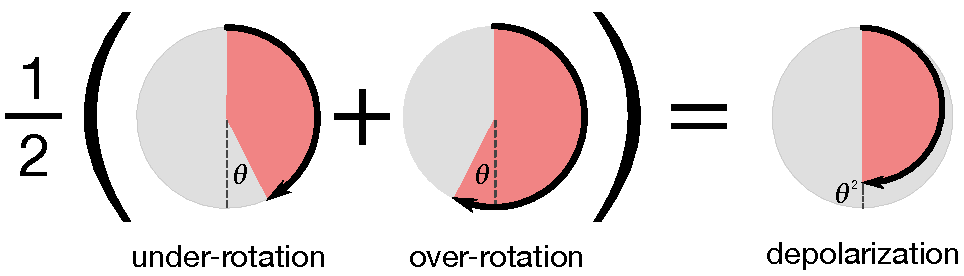
\includegraphics[width=\columnwidth]{simple_example.pdf}
  \caption{An example of a balanced control solution. Using optimal control, two implementations of a $Z_\pi$ gate are designed to have equal and opposite sensitivity to errors (if one implementation over-rotates by angle $\theta$, then the other \emph{under}-rotates by $\theta$). Each time the gate is used, one of these implementations is chosen at random. The resulting quantum channel is equivalent to a perfect implementation of the gate followed by dephasing of $\order{\theta^2}$.}
  \label{fig:simple_example}
\end{figure}

\section{Robustly Balanced Controls}
\note{Include the figure with the arrows and the derivation of the higher order terms and discussion that the optimal control that we're using is sufficient often to guarantee that the bare hamiltonian is asmall, so that we can take the expansion only to first order in delta in the easy way. Discuss the impact on diamond norm. We are going to use the mixing theorem from Campbell, so we'll have to quote that result. }
 Consider the problem of trying to approximate a target unitary operation, $U_T$. Define a control solution $c_i(t)$ by  \begin{equation}
\mathcal{T}e^{-i\int c_i(t)H(t, \vec{\delta})} = U_i \approx U_T
 \end{equation}
 where $\vec{\delta}$ are meant to be \textit{quasi-static}\cite{Ball2016} parameters of a Hamiltonian, $H(t, \vec{\delta})$. A family of control solutions is called a \emph{balanced control} if there is probability distribution $\vec{\omega}$ that satisfies the following for some small $\alpha$,
\begin{equation}\label{eq:1}
  \sum_{i=1}^N \omega_i U_i \rho U_i^\dagger = DPN[\alpha]\left(U_T \rho U_T^\dagger \right)
\end{equation}

where $\vec{\omega}$ must be a proper probability distribution and $DPN[\alpha](\rho)$ is a depolarizing noise channel, with strength $\alpha$. A depolarizing channel is defined as:
\begin{equation}\label{eq:2}
  DPN[\alpha](\rho) \rightarrow (1-\alpha)\rho + \alpha\sum p_i \sigma_i\rho\sigma_i
\end{equation}
with $p_i$ summing to one.

This is equivalent to the condition given by Campbell in \cite{Campbell2017}, that there exist a weight such that

\begin{equation}\label{eq:campbell-condition}
\sum \omega_j H_j(t, \vec{\delta})|_{\delta=\vec{0}} = 0
\end{equation}
however we will generalize this condition to define an RBC. A balanced control is said to be robust to order $\ell$ if a generalized form of Equation \ref{eq:campbell-condition} holds, namely if for all $1 \leq j \leq \ell$:
\begin{equation}\label{eq:RBC}
\begin{gathered}
\sum_k\omega_k(\sum_{n=0}^j D^n_k)^j = 0\\
D^n_k = \frac{1}{n!}\frac{\partial^{n}}{\partial\delta_{i_1}...\partial\delta{i_n}}H_k(t,\vec{\delta})|_{\delta=\vec{0}}
\end{gathered}
\end{equation}
Where the first sum is meant to result from Taylor expansion, and therefore will require matrix reshaping. These conditions imply that an $\ell^{th}$ order RBC ($\ell$RBC) is insensitive to the $\ell^{th}$ order in drift in $\vec{\delta}$. To see this, write the error on each gate in the RBC as $U_j(\vec{\delta}) = exp(-i(\tilde{H}_j(\vec{0}) + \frac{\partial}{\partial\delta_i}\tilde{H}_j(d\delta_i) +  \frac{1}{2}\frac{\partial^2}{\partial\delta_i\partial\delta_k} \tilde{H}_j(d\delta_i d\delta_k) + ...)U_T$, where $\tilde{H}(\delta)$ generates the error $U_j(\vec{\delta})U_T^{\dagger}$ over variations in $\vec{\delta}$. Then, by Taylor expanding $U_j(\vec{\delta})U_T^{\dagger}$ one finds that the the first $\ell$ derivatives of an $\ell RBC$ will be zero.

In all of the above, we will be interested in the case where $\alpha \approx \epsilon^2$, with $\epsilon$ being diamond distance from each member of the RBC to $U_T$. Following from Lemma 2 in \cite{Campbell2017}, if $0\in $ Conv$[\{\tilde{H}_i(t, \vec{\delta})\}]$, where Conv is the convex hull of its arguments then we know that $\vec{\omega}$ exists that satisfies Equation \ref{eq:1}. Then, following from the mixing lemma proven by both Campbell and Hastings\cite{1612.01011}, we can bound the the diamond distance from a balanced control to $U_T$ by $\epsilon^2$. Moreover, by following a generalized version of the algorithm Campbell presents in \cite{Campbell2017}, we can find families of controls that are $\ell$RBCs, for any $\ell$. In this setting, we can relax Equation \ref{eq:RBC}, to be
\begin{equation}\label{eq:RBC-relaxed}
\begin{gathered}
\sum_k\omega_kD^n_k = 0\\
\end{gathered}
\end{equation}
In this context, since we are assuming that the derivatives are all of norm $\epsilon$, the above condition guarantees that the error unitary be no worse than $\sum^n\epsilon^2\delta^n$ near the origin -- all orders can be quadratically supressed.
\section{A Simple Example}
\note{This particular instance is NOT robust, but we can construct one that IS. }
As a trivial example, consider a single-qubit rotation-angle error, such as from stochastic laser amplitude fluctuations. An RBC may consist of an $X_\pi$ pulse, as well as an $X_{-\pi}$ pulse (i.e., a clockwise and counter clockwise rotation of the qubit). In the case of excess amplitude, the $X_\pi$ pulse will result in an over-rotation error, while the $X_{-\pi}$ pulse will result in an \emph{under}-rotation error. When it comes time to perform the target gate in a quantum circuit, one member of the RBC is chosen uniformly at random. This has the effect of decreasing the norm of the noise channel and decorrelating the over-rotation error (Figure \ref{fig:simple_example}). In this simple example, we can analytically find a solution to Equation \ref{eq:1}. Specifically, by choosing weights $\omega_i=\frac{1}{2}$, we see:

\begin{equation}
  \begin{gathered}
    \frac{1}{2}(X^*_{\pi + \epsilon}\otimes X_{\pi + \epsilon} + X^*_{-(\pi + \epsilon)}\otimes X_{-(\pi + \epsilon)})) \\
    = (\sin^2{\frac{\pi + \epsilon}{2}}I\otimes I + \cos^2{\frac{\pi + \epsilon}{2}}X\otimes X)X\otimes X \\
    \approx DPN[\epsilon^2]X\otimes X
  \end{gathered}
\end{equation}

Therefore, for a rotational error of angle $\epsilon > 0$, we see that $X_\pi$ and  $X_{-\pi}$  form a 0RBC, with $\alpha\approx\epsilon^2$.

If we consider the amplitudes to not only be miscalibrated, but also non-Markovian (i.e. such that $\epsilon$ is drifting), we find the following channel, for any drift $\delta$:

\begin{equation}
  \begin{gathered}
  DPN[(\epsilon + \delta)^2]X\otimes X
  \end{gathered}
\end{equation}

Thus, the noise is always depolarizing, for every $\ell > 0$, this family of controls is an $\ell$RBC, and by injecting additional randomness the error rate is supressed quadratically.

\section{Optimal Control Problems}\label{ocp}
\subsection{Random Gate Synthesis}
 Generating RBCs can be done in a variety of ways, in this paper we consider using optimal control. In particular, one could use any of the many available quantum optimal control techniques \cite{Khaneja2005, Caneva2011, Machnes2018}. For our numerics, we chose to use the GRAPE algorithm. First described in \cite{Khaneja2005}, the GRAPE (GRadient Ascent Pulse Engineering) algorithm is a technique for finding piecewise constant control sequences that approximate a desired unitary, $U_T$. Defining the uncontrolled Hamiltonian as $H_0$, the control Hamiltonians as $H_{i\neq 0}$, and the \textit{control matrix} $c_{ij}$ as containing control amplitude associated with the $i^{th}$ time step and the $j^{th}$ hamiltonian, we can write an approximate unitary for any timestep of evolution as:
\begin{equation}\label{eq:3}
  U_i = \exp\{-i\Delta t(H_0 + \sum_{j=1}^{n}c_{ij}H_{j}\}
\end{equation}
Then, to measure the simularity of our approxiate unitary $U=\prod_iU_{i=1}^n$ to our target unitary $U_T$, we can define a cost function $J(U) = Tr\{U_T^{\dagger}U\}$.

To optimize this cost function we can perform the following standard update loop for some threshold value $\varepsilon > 0$ and step size $\delta > 0$:
\begin{algorithm}[H]
\floatname{algorithm}
  \caption{\textsc{\textbf{Gradient Ascent}}}
  \begin{algorithmic}
    \While{$J(U) < (1-\varepsilon$)}
    \State $c_{ij} \rightarrow c_{ij} + \delta\frac{\partial J(U)}{\partial c_{ij}}$
    \For{$1 \leq i \leq n$}
    \State $U_i \rightarrow \exp\{-i\Delta t(H_0 + \sum_{i=0}^{n}c_{ij}H_j)\}$
    \EndFor
    \State $U \rightarrow \prod_{i=1}^nU_i$
    \EndWhile
  \end{algorithmic}
\end{algorithm}

In general these gradients can be computed by propagating partial derivatives of the cost function with respect to control parameters through each timestep of the  via the chain rule. However, in \cite{Khaneja2005} Khaneja et al. derive a simple update formula that is correct to first order. In particular one can show that:
\begin{equation}\label{eq:update}
  \begin{split}
\frac{\partial J(U)}{\partial u_{ij}} = -2Re\{\braket{{U_{j+1}^{\dagger}...U_N^{\dagger} U_T}}{i\Delta tH_jU_j...U_1}\\
\braket{U_j...U_1}{U_{j+1}^{\dagger}...U_N^{\dagger} U_T}\} +  \mathcal{O}(\Delta t^2)
  \end{split}
\end{equation}

Because we our trying to generate high-order RBCs, we want to generate controls that perform well over a wide range of parameter values ($\delta$). To do this, we modified the gradient in GRAPE to instead be:
\begin{align}\label{quadrature}
\frac{\partial \tilde J(U)}{\partial u_{ij}} =
\int p(\vec{\delta})\frac{\partial J(U(\vec{\delta}))}{\partial u_{ij}} d\vec{\delta}
\end{align}
with $p(\vec{\delta})$ Gaussian distributed, as has been done in previous works \cite{Goerz2014} to ensure that the optimal control results are robust over a wide range of errors. To make this averaging tractable, we approximate this integral using Gaussian quadrature, approximating the cost functions as a low order polynomials\cite{abramowiz1972handbook}.
\note{Discuss how this is a proxy for the higher-order derivatives being small. Discuss the difference between the step control functions and the cost function in the optimization.}

\subsection{RBC Approximation}
After using GRAPE or another optimal control routine to synthesize a collection of controls, we must find the weights $\omega_i$ such that the collection of controls form an $\ell$RBC as described in Equation \ref{eq:RBC}. To do this, for each control $U_i(\vec{\delta})$ we find the unitary error channel $\mathcal{E}_i(\vec{\delta})$ such that $\mathcal{E}_i(\vec{\delta})U_i(\vec{\delta})=U_T$, where $U_T$ is the target gate. By taking the logarithm of these error maps, we then get a family of Hamiltonians $\tilde{H}_j(\delta)$, and conside the following quadratic program whose solutions satisfies the robustness conditions given in Equation \ref{eq:RBC}. Namely:
\begin{equation}\label{eq:minimization}
  \begin{split}
    &\textbf{minimize: } ||D_{\ell}^T\omega||\\
    &\textbf{subject to: } \forall i<\ell,\ D_i=0\\
   	&\phantom{\textbf{subject to: }}\sum \omega_j = 1\\
   	&\phantom{\textbf{subject to: }}\sum 0 \le \omega_j \le 1
  \end{split}
\end{equation}
%These constraints for each $P_i$ can be broken into $2_{\ell-1}$ constraints, one for the imaginary components, and one for the real component. Alternatively, one can express the Hamiltonians as vectors in $\mathbb{R}^{2^n}$

The question still remains -- when does this quadratic program have a solution. Naturally, if the control family is too small a solution won't exist. As in \cite{Campbell2017}, we need  $0\in $ Conv$[\{\frac{\partial^{\ell}}{\partial\delta_{i_1}...\partial\delta{i_\ell}}\tilde{H}_j(t,\vec{\delta})|_{\vec{\delta}=0}\}]$. This can be accomplished by modifying the oracle in Campbell's algorithm to produce robust controls, in particular by updating the GRAPE cost function to include derivative information, one could produce controls with derivatives of order $\epsilon$. Finally one would like to ensure that the control family produced is not too large - that is given the family of controls, we would like to regularize the cost function to enforce sparsity. In this case, lasso regularization is insufficient as we already constrain the one norm of the vector we optimize over to be unity. However, the problem of enforcing sparsity in such situations has been considered in \cite{NIPS2012_4504} and remains a convex problem.

%In addition, for the constraints to be feasible, it is clear that the following condition is necessary: take $dim(\omega)=\Omega$, and $dim(\delta)=\Delta$. Each constraint is a matrix with $\Delta^i2^n$ elements. Thus we need at least $\Delta^i2^n$ linearly independent controls to even span the space of feasible weight vectors. On the other hand, even if the controls span the space, this is not sufficient because they must contain the origin in their complex hull. This can be achieved via a generalization of Campbell's Algorithm and by modifying the oracle query to ask for controls whose derivatives also satisfy certain properties.


Previous authors have considered minimizing the diamond distance to the nearest Pauli or Clifford Channel \cite{Magesan2013}, and while this gives a good theoretical framework it does not constrain the resulting channel to be decomposable into a given family of controls. Our routine, on the other hand, produces a channel defined explicitly in terms of given family of controls.

% \begin{figure*}
% \centering
% \begin{subfigure}[t]{.5\linewidth}
% 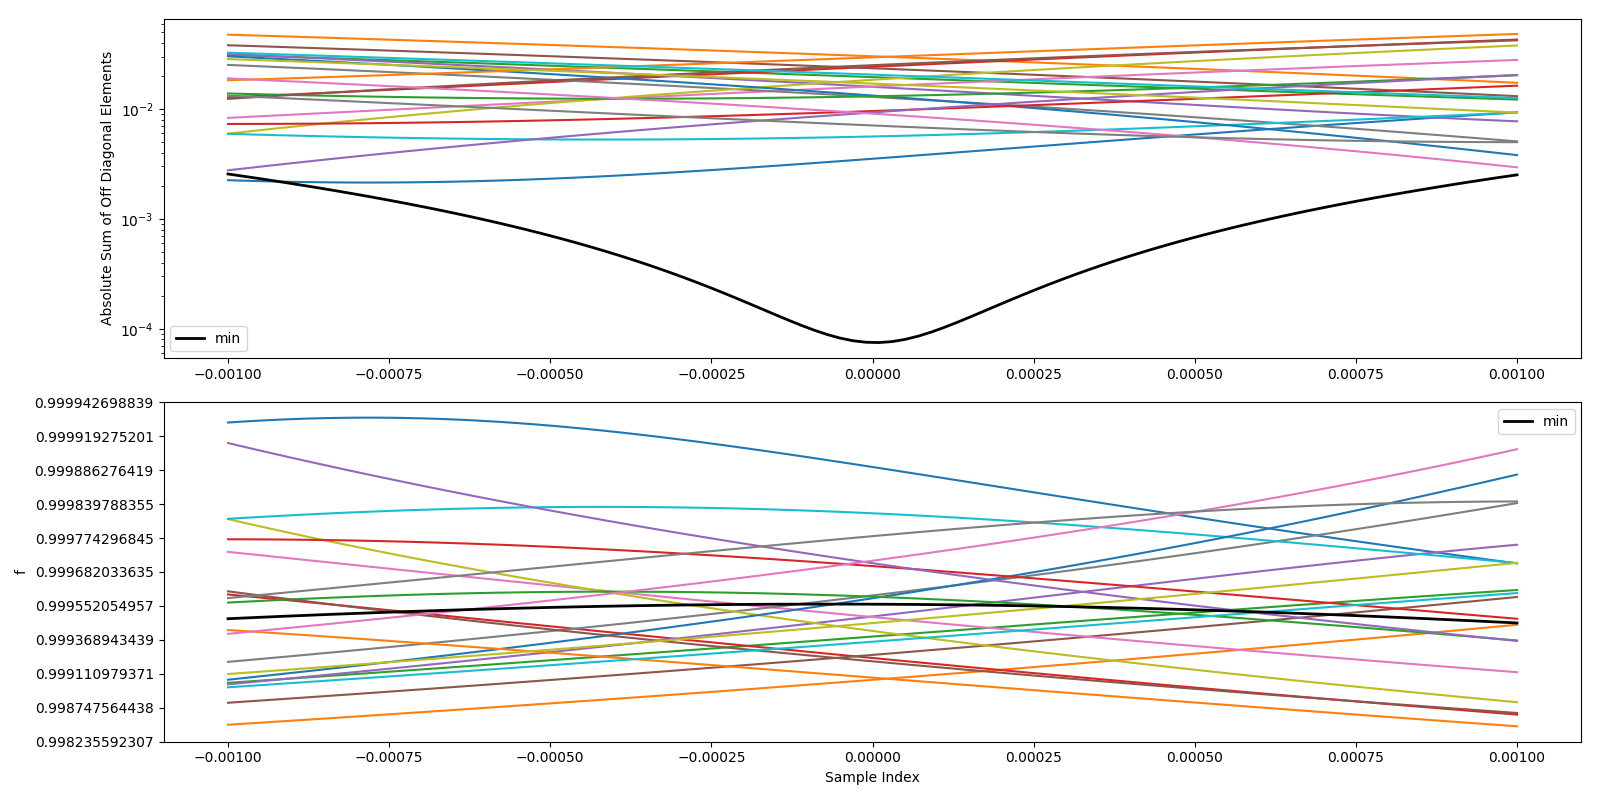
\includegraphics[width=\textwidth]{1q0.png}
% \caption{This is one example of a 1D slice varying over one control.}
% \end{subfigure}%
% ~
% \begin{subfigure}[t]{.5\linewidth}
% 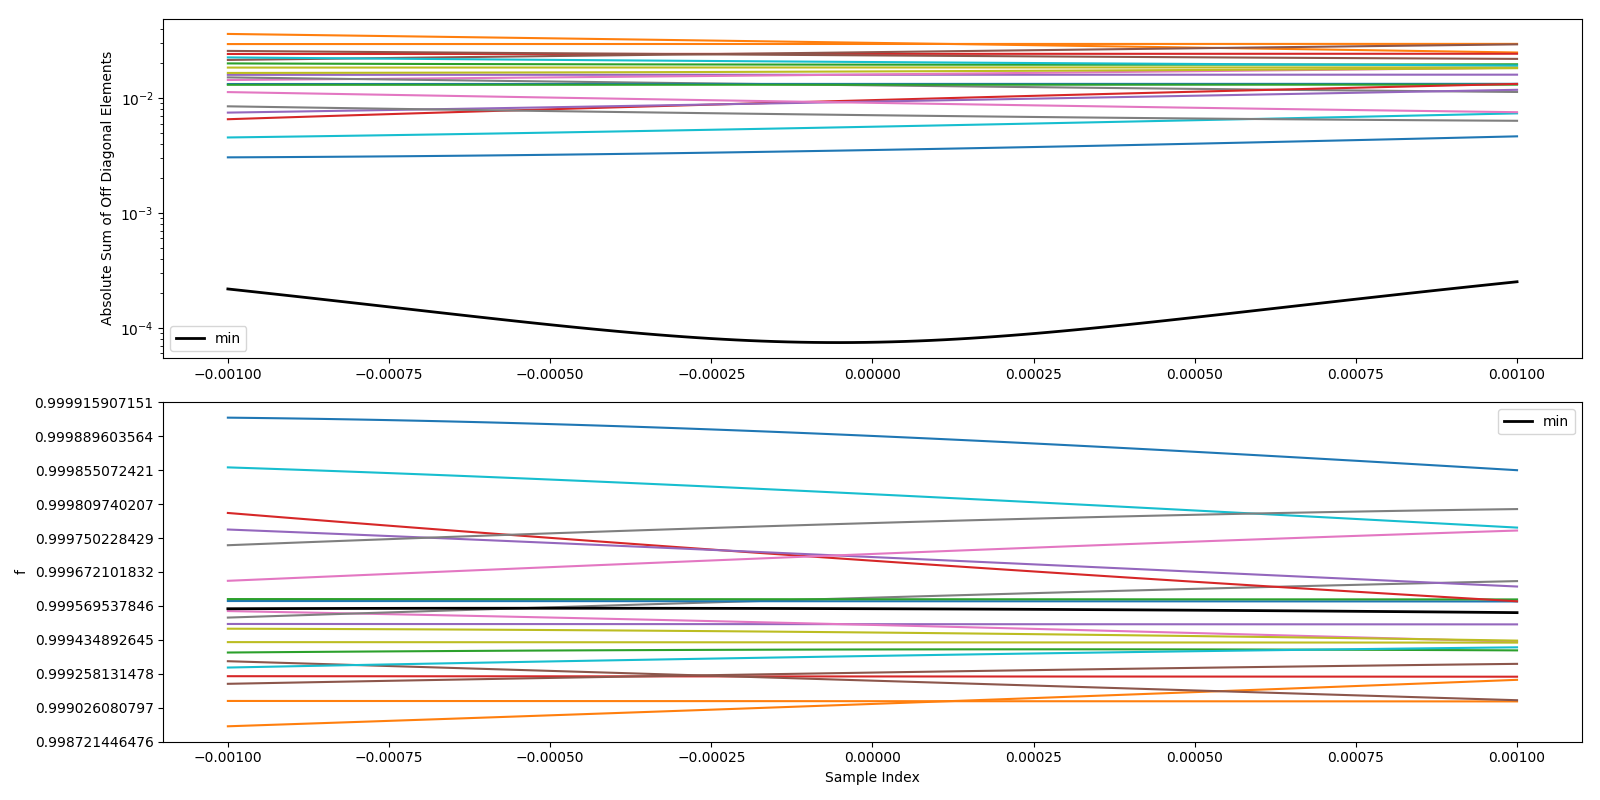
\includegraphics[width=\textwidth]{1q1.png}
% \caption{This is another example of a 1D slice varying over one control.}
% \end{subfigure}
%   \label{fig:1qnum}
% \end{figure*}



% \begin{figure*}
% \centering
% \begin{subfigure}[t]{.5\linewidth}
% 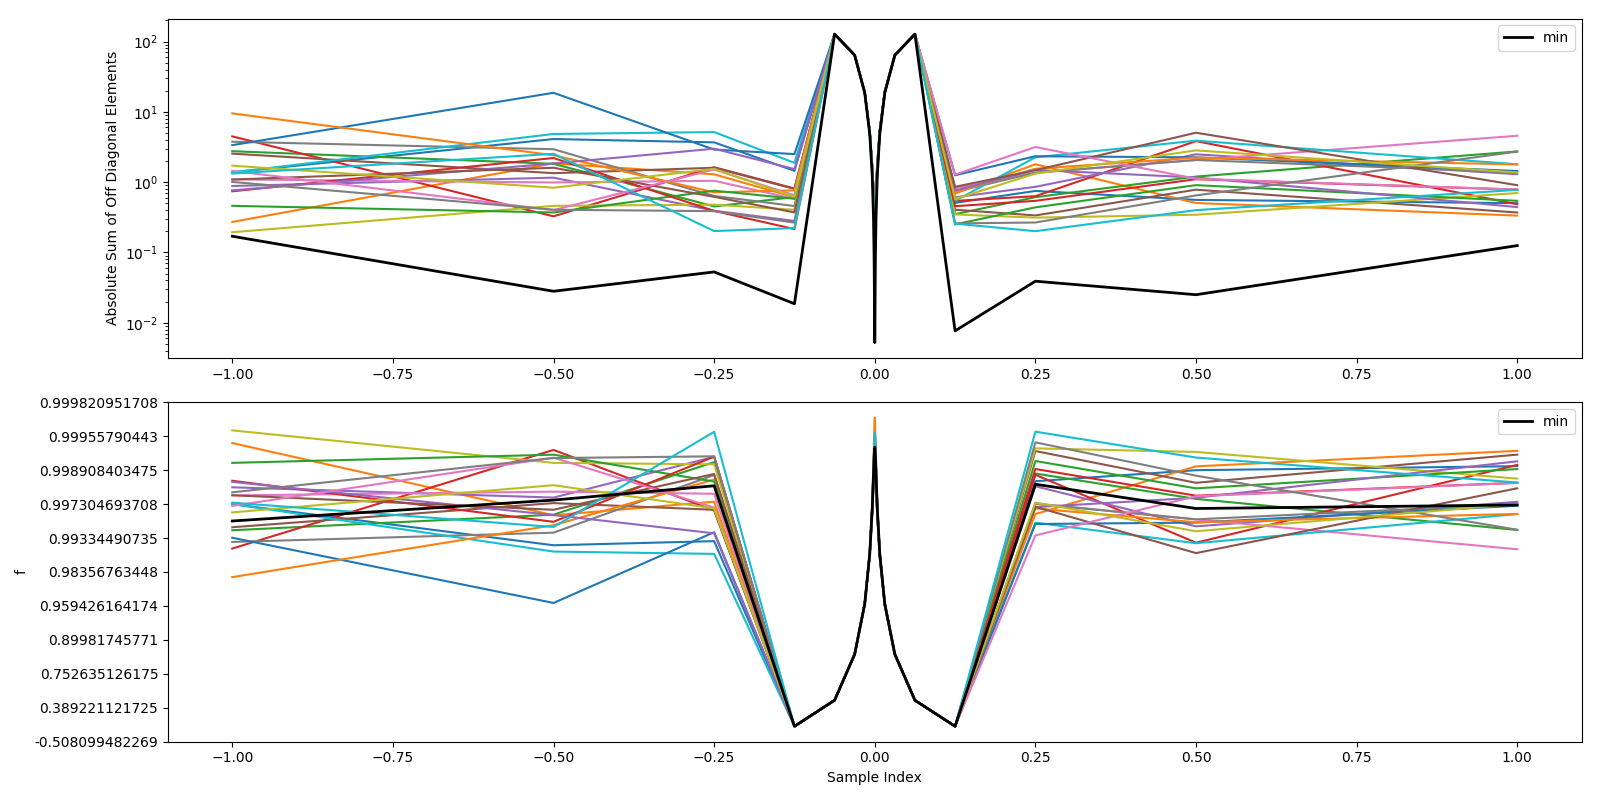
\includegraphics[width=\textwidth]{control_dpn_all0.png}
% \caption{This is one example of a 1D slice varying over one control. There are five of these in total, but only one is interesting.}
% \end{subfigure}%
% ~
% \begin{subfigure}[t]{.5\linewidth}
% 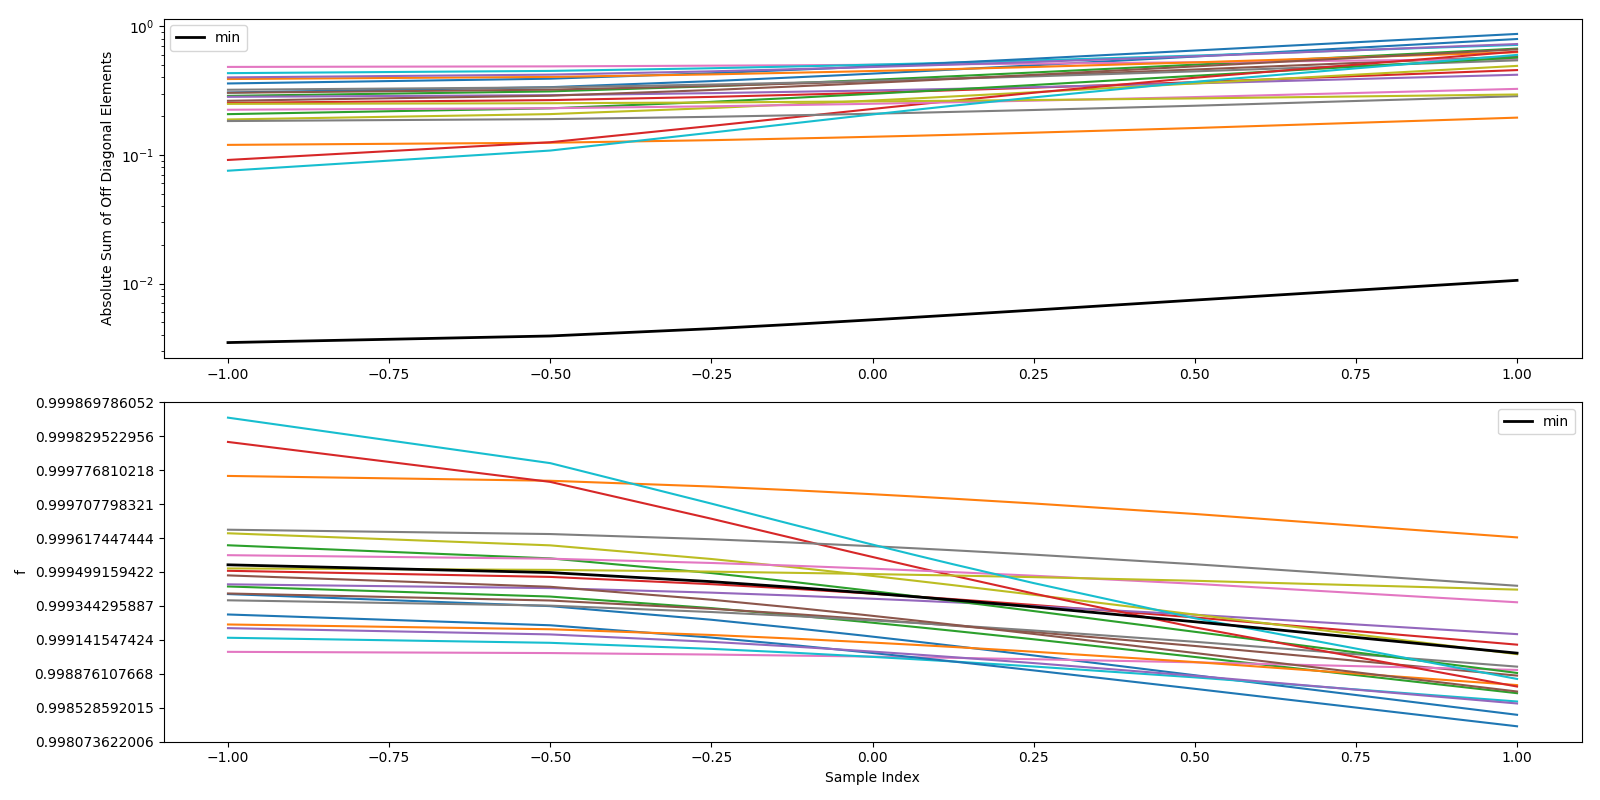
\includegraphics[width=\textwidth]{control_dpn_all2.png}
% \caption{This is one example of a 1D slice varying over one control. There are five of these in total, but only one is interesting.}
% \end{subfigure}
%   \label{fig:2qnum}
% \end{figure*}

\section{Numerical Results}\label{numerical}
In the following two subsections, we present numerical results of our routine, first for a one qubit example, and then for a two-qubit example. The code and RBCs generated for both examples are available online at \cite{decorrelating_errors}.
\subsection{1Q Gates}\label{1Q Gates}
 For the one-qubit case, we generate a 1RBCs for $RX(\frac{\pi}{2})$. Our control Hamiltonian is given as:
\begin{equation}\label{eq:1Qham}
  H(\delta, \epsilon, t) = \epsilon\sigma_z + (1 + \delta)(c_x(t)\sigma_x + c_y(t)\sigma_y)
\end{equation}
where we take  when generating the members of the RBC. We assume that the errors on $\sigma_x$ and $\sigma_y$ are perfecly correlated, as mentioned in Section \ref{ocp}. When generating the controls, we chose an total evolution time of $T=\pi$, a number of steps $N=100$, and a threshold infidelity of $1E-3$, with $\epsilon, \delta \sim \mathcal{N}(0, .001)$. The results can be seen in \ref{fig:num}. In particular, over a wide region about the origin, the diamond norm can be seen to have been reduced by over an order of magnitude.

\begin{figure}\label{fig:num}
  \centering
  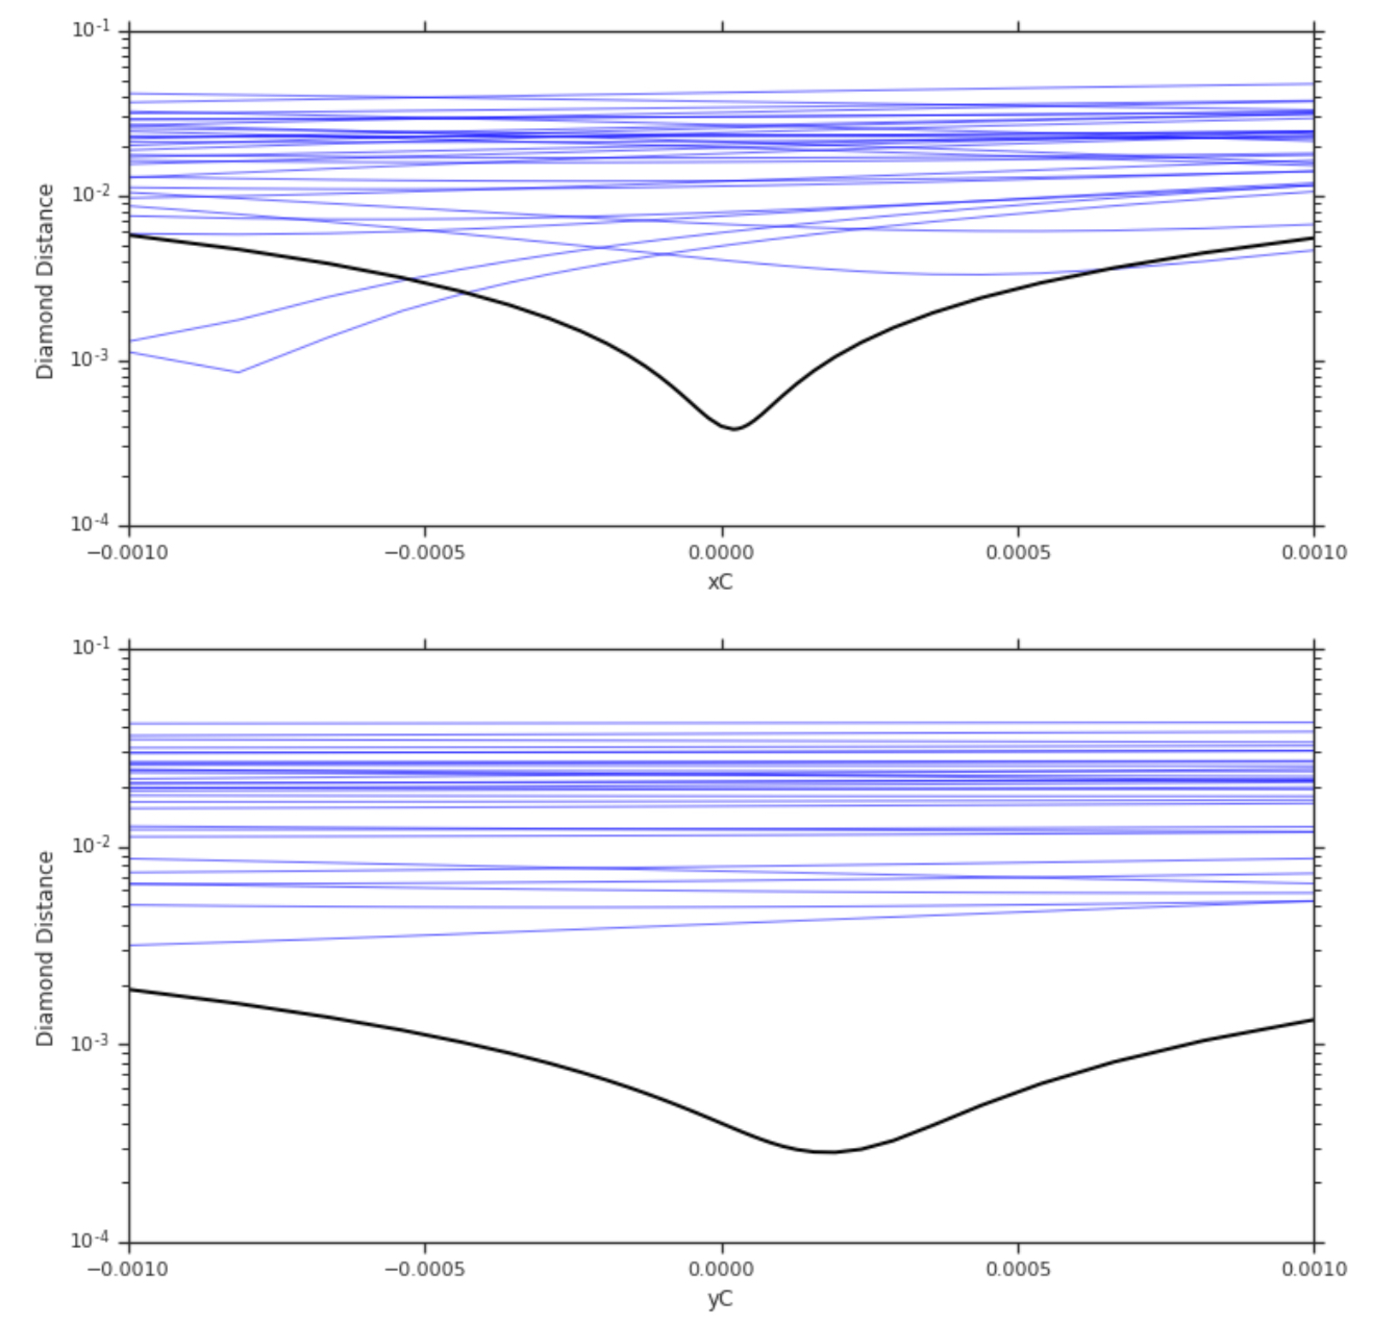
\includegraphics[width=\columnwidth]{placeholdernumerical.pdf}
  \caption{Placeholder image until we figure out what to plot. This currently shows that for one of the control the diamond norm decreased by over an order of magnitude. The labels need to be bigger.}
  \label{fig:rb}
\end{figure}
%The results can be seen in \ref{fig:1qnum}, where we have plotted each control as a function of one detuning value, fixing the others to zero. In the top half of each plot, we show the variation in the sum of the absolute valua of the off diagonal elements of the Pauli-Liouville Representation, while in the lower plot we see the variation in fidelity. While the controls were optimized by considering Gaussian noise with $\sigma=.001$ for each control, we have plotted the performance of the controls over a wider range to show more structure. We see over an order of magnitude improvement in the sum of the absolute values of the off-diagonal elements, while the fidelity remains above the specified target.



\subsection{2Q Gates}\label{2Q Gates}
 For a two-qubit example, we chose $ZZ(\frac{\pi}{2})=\exp{(-i\frac{\pi}{4}\sigma_z\otimes\sigma_z)}$. Our control Hamiltonian is given as:
\begin{equation} \label{eq:2Qham}
\begin{split}
H(\vec{\epsilon}, \vec{\delta}, \eta, t) = &\sum_{j=1}^2(\epsilon_j\sigma_z^j + (1 + \delta_j)(c_x^jx(t)\sigma_x^j + c_y^j(t)\sigma_y^j)) \\
&+ (1+\eta)c(t) \exp{(-i\frac{\pi}{4}\sigma_z^1\otimes\sigma_z^2})
\end{split}
\end{equation}
We again consider $\epsilon_j, \delta_j, \eta \sim .001$, however and a threshold infidelity of $1E-3$, however we increased the total evolution time to $T=4\pi$, and increased the number of steps to $N=400$ so that the size of each time step was the same as in the one qubit example and so that the total evolution time was greater to allow GRAPE more opportunities to find non-trivial pulseshapes. The results also show a reduction of an order of magnitude in diamond norm about the origin, and for a wide neighborhood around it.

%0.0507,  0.0307, -0.0493, -0.0693, with total area under the curve given by 0.7853981633974484,
\section{Experimental Results}\label{experimental}
Here we present experimental results from implementing our routine on a fixed-frequency superconducting transmon qubit. In particular we used qubit 8 on the Rigetti 19Q-Acorn chip, whose characterization can be found in \cite{1712.05771}. To implement a RBC on this qubit, four incorrectly calibrated approximately Gaussian pulses were produced by scaling the pulseshape for a calibrated 50$\mu$s $RX(\frac{\pi}{2})$ pulse by $106.4\%$,  $103.9\%$, $93.7\%$ and $91.2\%$.

 Using Equation \ref{eq:minimization}, we then generated the optimal weighting $\omega_i$. To benchmark the quality of the new balanced channel, we then performed six randomized benchmarking experiments: one for each over- and under-calibrated pulse, one for the calibrated pulse, and one for the balanced channel. We used $N=1000$ shots per experiment and $K=10$ sequences per sequence length, for sequence lengths up to $L=64$\cite{Magesan2011}. In each case, our Clifford operations were decomposed into RX($\frac{\pi}{2})$) and RY($\frac{\pi}{2})$) pulses. In our implementation, these gates are implemented using the same pulse envelope definitions and control electronics, phase shifted by $\frac{\pi}{2}$ radians, and are therefore subject to identical miscalibration errors. The results are shown in Figure \ref{fig:rb} for sequence lengths $L=64$.

%with scipy's curve\_fit using the Trust Region Reflective method
In this experiment, fitting the randomized benchmarking data reports one-qubit gate fidelities of $99.4\%$ for the calibrated pulse, $98.8\%$ for Pulse1, $99.4\%$ for Pulse2, $98.9\%$ for Pulse3, $98.6\%$ for Pulse4, and $99.0\%$ for the Randomized pulse. However, as one can see from looking at Figure \ref{fig:rb}, despite all controls performing comparably to the Calibrated control, only the Randomized control has similarly tight error bars. In the cases of each miscalibrated pulse, the error bars extend significantly, in often asymmetric ways, making usage of chi-square statistics, and errors on the fit less straightforward.

This is consistent with the result shown in \cite{Ball2016} that for particular non-Markovian error models, noise will manifest as gamma distributed points for each sequence length. On the other hand, Markovian noise, such as depolarizing noise, will result in Gaussian distributed fidelity estimates for each randomized benchmarking sequence length. We see that the coherently miscalibrated controls have long tails, consistent with gamma distributed random variables, while the calibrated and randomized implementations both have much shorter tails, consistent with Gaussian distributed random variables.

\begin{figure}
  \centering
  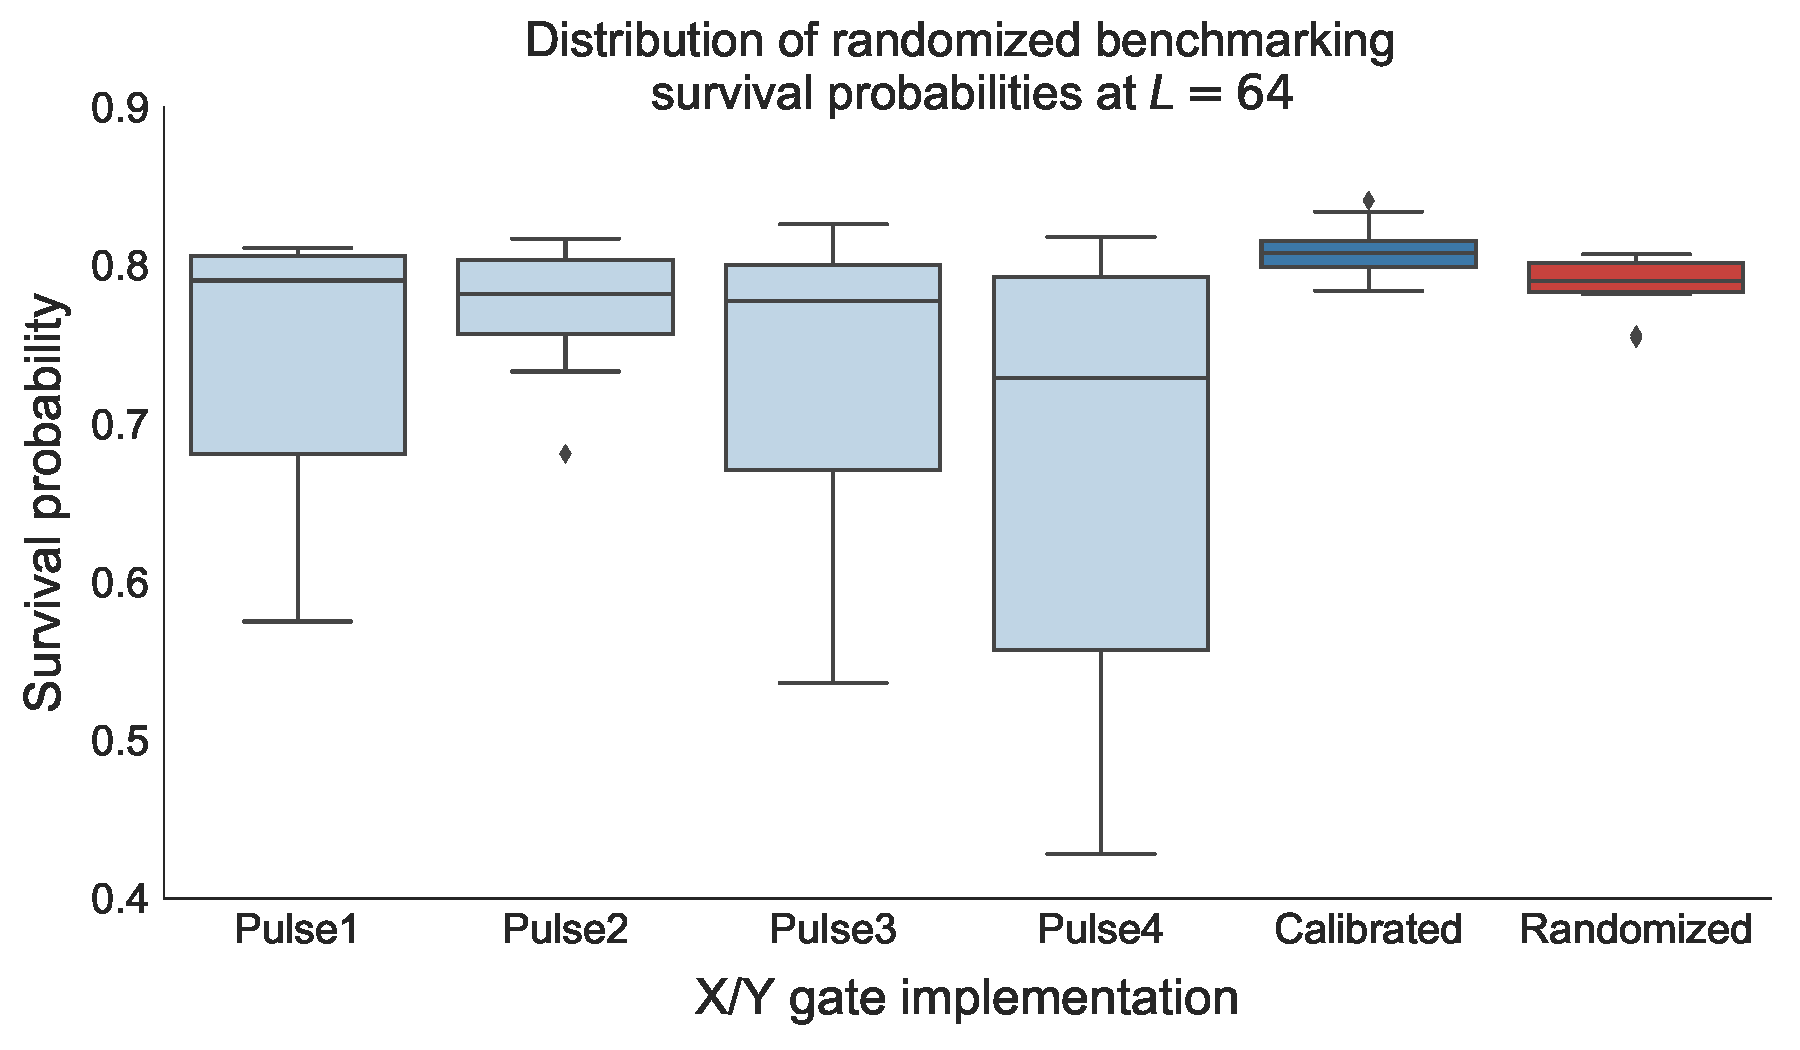
\includegraphics[width=\columnwidth]{rb_data.pdf}
  \caption{Randomized benchmarking experiments ran using different pulse definitions. The four plots on the left are from the incorrectly calibrated pulse, while the top right is the calibrated pulse, and the bottom right is the BCS.}
  \label{fig:rb}
\end{figure}

\section{Conclusion and Future Work}
We have shown numerically that using RBCs can reduce non-Markovian, coherent error on a quantum channel by more than an order of magnitude in diamond norm, over a wide range of quasi-static values of noise. In addition, we have demonstrated that these approximate controls can be generated through optimal control (GRAPE), and that the minimization problem is tractable.

%Contrasting with \cite{Ware2018}, we see that this method of non-Markovian and coherent error mitigation is cheap to implement - it only requires a random choice of pulse definition at run time, in addition to the extra storage required to store the pulse definitions. In particular, no classical preprocessing or runtime frame tracking is required.

Future directions for this work include demonstrating the routine experimentally on a two-qubit gate, moving the random gate selection from a precompilation step to runtime logic onboard the FPGA, investigating other optimization routines such as CRAB \cite{Caneva2011} and GOAT\cite{Machnes2018}, and using more sophisticated benchmarking routines such as GST\cite{BlumeKohout2017} to quantitatively investigate the performance of our method.

Another interesting area of research would be using model-free approaches. The numerical work in the paper assumes access to a model of the system, however an experimentalist may not have a model readily available to describe the system, e.g. in the presence of unknown on-chip crosstalk, or an uncalibrated transfer function of the system. Moreover, even if a model is available, it might be computationally inconvenient to simulate, i.e. for more than a few qubits.%, or for non-adiabatic gates, where the timestep is required to be much smaller than the gate-time.

In these situations, one approach would be to use \textit{in-situ} optimal control techniques \cite{Wu2018, Kelly2014, Ferrie2015} to generate candidate controls, and then use an optimizer like Nealder-Mead to perform the minimization. While performing a complete optimization in this way would still be slow, requiring full process tomography, one could intead optimize via partial tomography. By selecting pre-- and post --rotations that correspond to measuring pauli moments of interest in the Hamiltonian, such as unwanted $Z\otimes Z$ crosstalk, one could perform optimization over fewer parameters.

\section{Acknowledgements}
Sandia National Laboratories is a multimission laboratory managed and operated by National Technology and Engineering Solutions of Sandia, LLC, a wholly owned subsidiary of Honeywell International, Inc., for the U.S. Department of Energy's National Nuclear Security Administration under contract DE-NA0003525.
\bibliography{decorrelation.bib}
\end{document}
